% just like python and another other programming language
% we must load our packages and setup the document

\documentclass{beamer} % I want to make a presentation

\usepackage[utf8]{inputenc}
\usepackage{amsmath, amssymb}
\usepackage{graphicx}
\usepackage{url}
\usepackage{float}

\usepackage{longtable} % Required for the longtable environment
\usepackage{array} % Required for custom column specifications
\usepackage{calc} % Required for calculations
\usepackage{ragged2e} % Required for \raggedright in column specification
\usepackage{booktabs} % Required for \toprule, \midrule, \bottomrule


%\usepackage[style=apa, doi=true, backend=biber]{biblatex}
%\DeclareLanguageMapping{american}{american-apa}
%\addbibresource{sources.bib}

% this section contains everything needed for titling and headers

% the following contains our abstract/aka the draw
%\keywords{keyword1, keyword2}
%\abstract{ABSTRACT TEXT HERE}

% PRESENTATION NOTES
% keep it simple, 




\usetheme{default}  % Replace "YourTheme" with the desired theme (e.g., "Madrid", "Berlin", "CambridgeUS")



% Set the title, author, and date
\title{Examining Housing Instability Trends and the Moderating Impacts of the Covid-19 Eviction Moratorium in San Diego County}
\author{Kaye Prosser, Andrew Lona}

%\affiliation{{University of California, San Diego}}
%\authornote{Special thanks to our capstone advisors, Dr. Jennifer Nations and Julie Wartell.}
\date{\today}

\begin{document}
  
% Title slide
\begin{frame}
  \titlepage
\end{frame}


% RUBRIIC

% Section 1
% What questions motivated your work

\begin{frame}
\frametitle{Research Question}

What factors influenced housing instability before, during, and after Covid-19 eviction moratorium in San Diego county? If any, which trends could best explain these differences across the county? In order to answer these questions we are using two approaches for estimating housing instability. 

\end{frame}


% Section 2
% What data you analyzed

\begin{frame} 
\frametitle{Data}

Two data sets:

\begin{itemize}
	\item Forced Eviction-lockout data
	\begin{itemize}
		\item Created by joining data from ZCTA renter household occupancy and Forced Eviction lockout reports from the court. 
	\end{itemize}
	
	\item Community Information Exchange (CIE) data
	\begin{itemize}
		\item Demographic data of need-determined 2-1-1 callers by network members. 
	\end{itemize}
\end{itemize}
\end{frame}


\begin{frame}
\frametitle{Data}
\framesubtitle{Evictions}

\begin{figure}[H]
  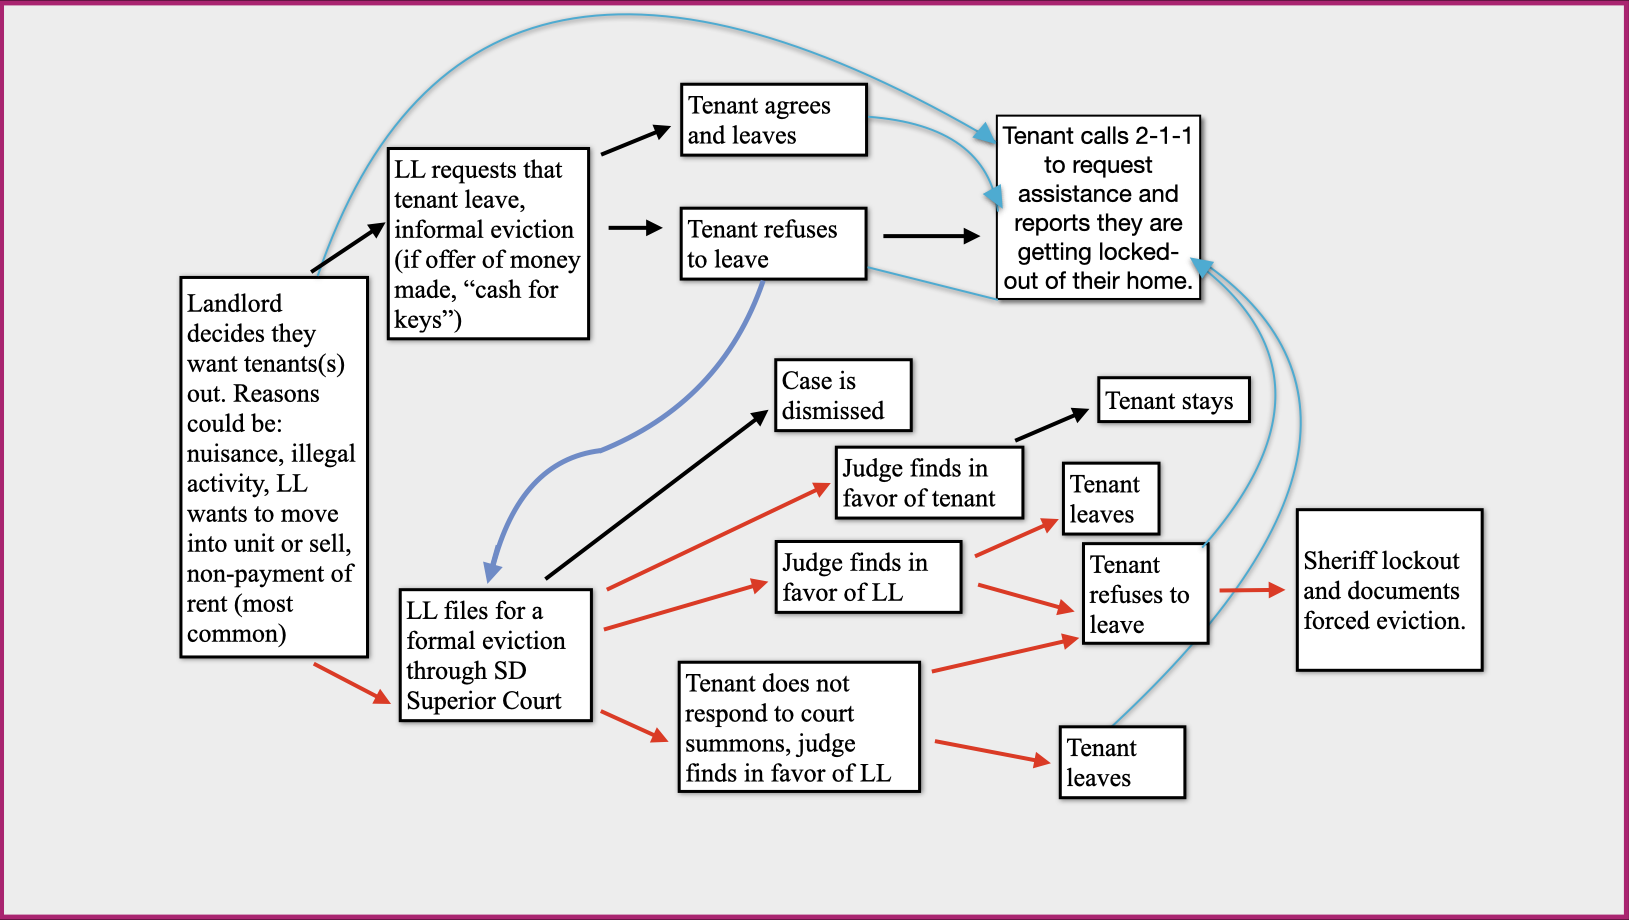
\includegraphics[width=\linewidth]{figures/housing_precarity_tree.png}
  %\caption{Illustration of Housing Precarity Ties.}
  \label{fig:housing_precarity_tree}
\end{figure}

\end{frame}

% For CIE demographics needs
\begin{frame}
\frametitle{Data}
\framesubtitle{CIE Needs}
\begin{figure}
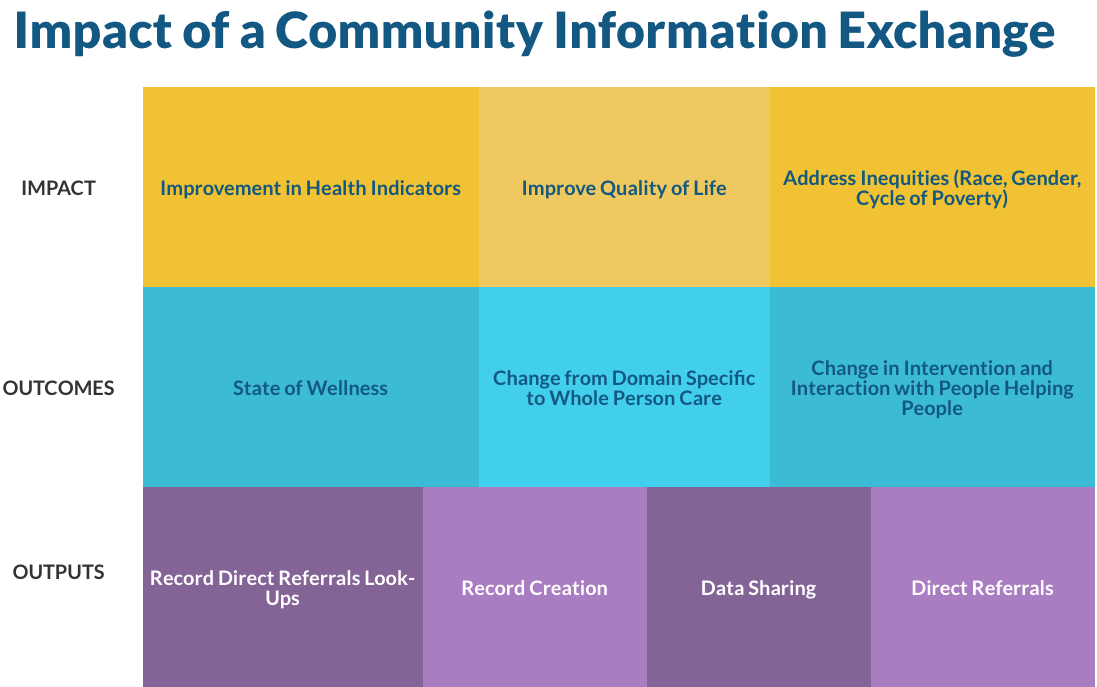
\includegraphics[width=0.85\linewidth]{figures/impact_CIE.png}
\end{figure}

\begin{enumerate}
	\item Caller dials 2-1-1 and speaks to representative.
	\item Caller is recorded in CIE network, directed to partner.
	\item Partner evaluates and determines need, can redirect to another partner.
\end{enumerate}


\end{frame}


% Section 3
% The basic method of data analysis you used

% For Evictions
\begin{frame}
\frametitle{Methods}
\framesubtitle{Evictions}

\begin{itemize}
\item Spatial Patterns in Residential Lockout Eviction Orders by ZIP code for San Diego County
\end{itemize}

\vspace{10pt} % insert formula
For each period ($p$) for each Zip/ZCTA ($z$):
$$evictionsrate = \frac{(evictionscounts_{zp}/rentalhouseholdoccupancy_{zp} * 1000)}{month_{p}}$$

\begin{figure}
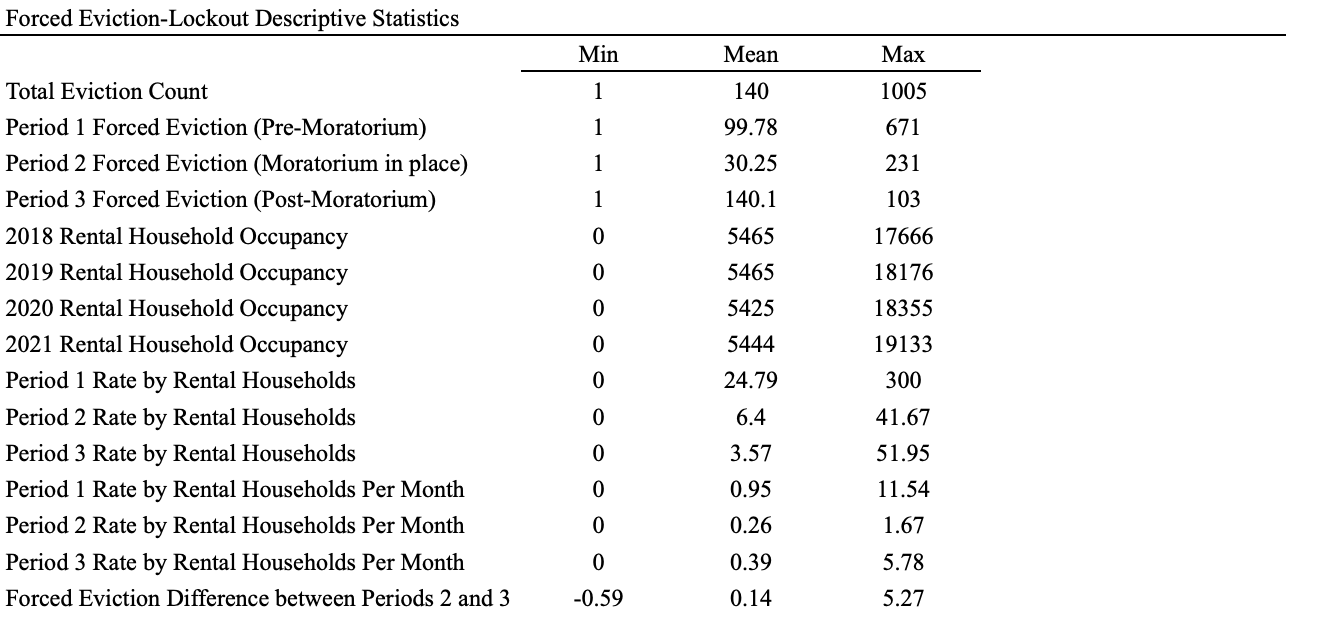
\includegraphics[width=0.85\linewidth]{figures/Table_1_FEviction_DescriptiveSTATS.png}
  %\caption{Forced Evictions Desc Stats}
  \label{fig:desc_stats}
\end{figure}
\end{frame}


% for CIE demographics needs
\begin{frame}
\frametitle{Methods}
\framesubtitle{CIE Needs}
\center
Poverty Rate $= \frac{{\text{Poverty}_{ZCTA, Year}}}{{\text{Population}_{ZCTA, Year}}} * 100$
\vspace{40pt}

For each need ($n_{i}$),

$ n_{i} = \beta_0 + \beta_1 \cdot Accounts\footnote{Gender, Age, Race/Ethnicity} + \beta_2 \cdot Poverty Rate + \beta_3 \cdot Moratorium Period + \epsilon$

\end{frame}




% Section 4
% Your most interesting or revealing findings, discussed in the context of your questions (This is a great opportunity to show off your favorite visualizations!)

% for Evictions
\begin{frame}
\frametitle{Results}
\framesubtitle{Evictions}
\begin{figure}[H]
  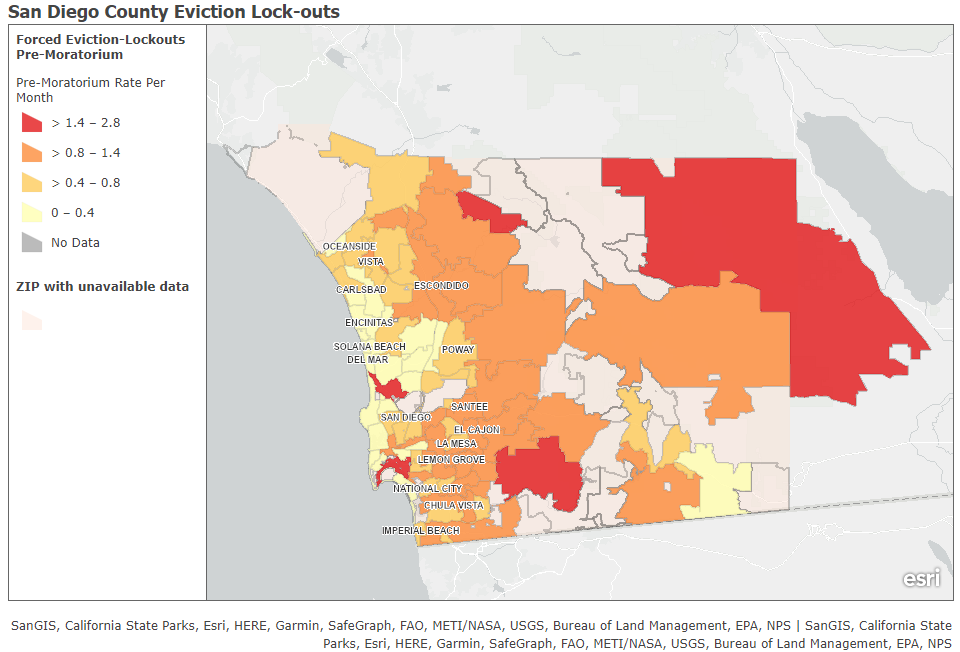
\includegraphics[width=0.85\linewidth]{figures/gis_pre_figure1.png}
  \caption{GIS Map of Forced Eviction-lockouts prior to the COVID-19 moratorium}
  \label{fig:pre-moratorium}
\end{figure}
\end{frame}

\begin{frame}
\frametitle{Results}
\framesubtitle{Evictions}
\begin{figure}[H]
  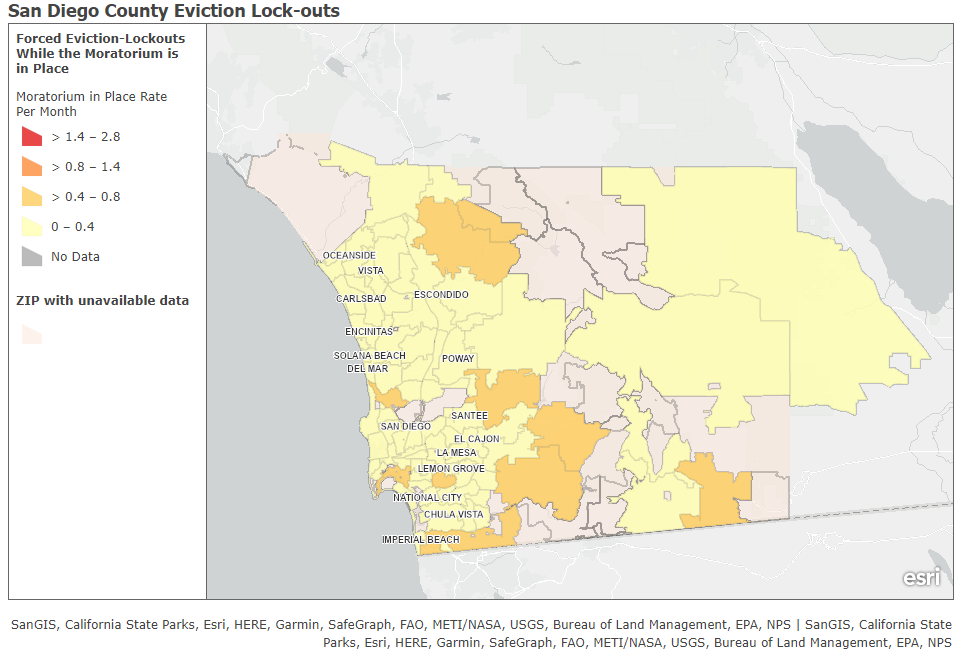
\includegraphics[width=0.85\linewidth]{figures/gis_during_figure2.png}
  \caption{GIS Map of Forced Eviction-lockouts with the COVID-19 moratorium in place}
  \label{fig:during_moratorium}
\end{figure}
\end{frame}

\begin{frame}
\frametitle{Results}
\framesubtitle{Evictions}
\begin{figure}[H]
  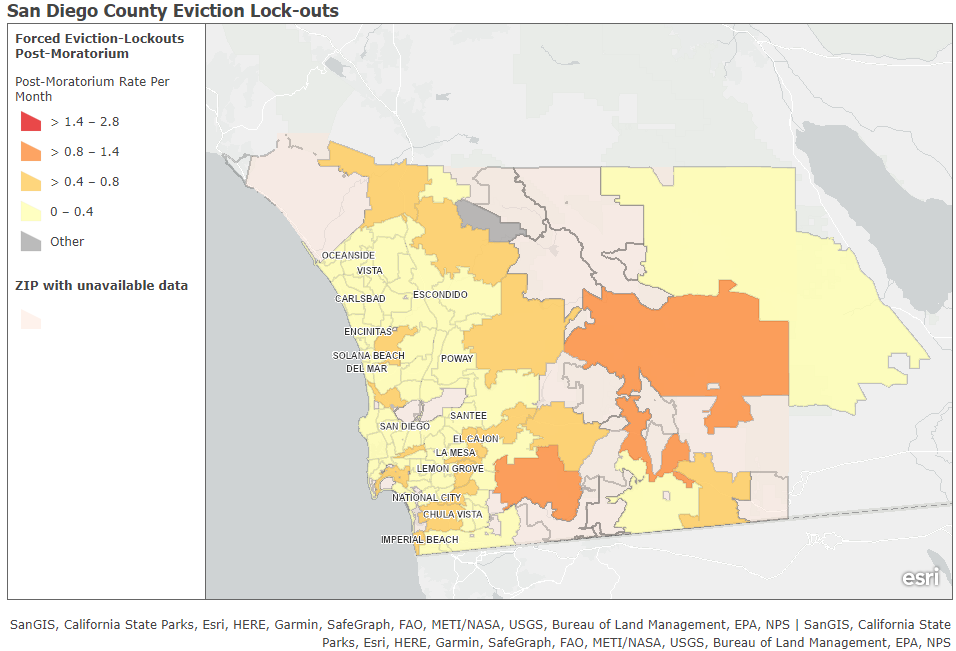
\includegraphics[width=0.85\linewidth]{figures/gis_post_figure3.png}
  \caption{GIS Map of Forced Eviction-lockouts POST COVID-19 moratorium}
  \label{fig:post_moratorium}
\end{figure}
\end{frame}



% for CIE demographics needs
\begin{frame}
\frametitle{Results}
\framesubtitle{CIE Needs}
\begin{table}[!htbp]
\centering
\caption{In-Sample Model Performance: AIC/BIC lower is better | LogLik higher is better}
\label{}
\resizebox{\linewidth}{!}{
\begin{tabular}{cccc}
\\[-1.8ex]\hline
\hline \\[-1.8ex]
& AIC & BIC & LogLik \\
\hline \\[-1.8ex]
Original Model $H_0$ (Housing Needs) & $27,328.6900$ & $27,415.7800$ & $$-$13,653.3400$ \\
Moratorium Added $H_1$ (Housing) & $42,199.7200$ & $42,286.8100$ & $$-$21,088.8600$ \\
Original Model $H_0$ (Utilities Needs) & $26,011.0100$ & $26,098.1000$ & $$-$12,994.5100$ \\
Moratorium Added $H_1$ (Utilities) & $39,060.9000$ & $39,147.9900$ & $$-$19,519.4500$ \\
\hline \\[-1.8ex]
\end{tabular}
}
\end{table}
\end{frame}

\begin{frame}
\frametitle{Results}
\framesubtitle{CIE Needs}
ROC/AUC Out-Of-Sample Model Performance | R = 5, K = 50.
\begin{figure}[H]
  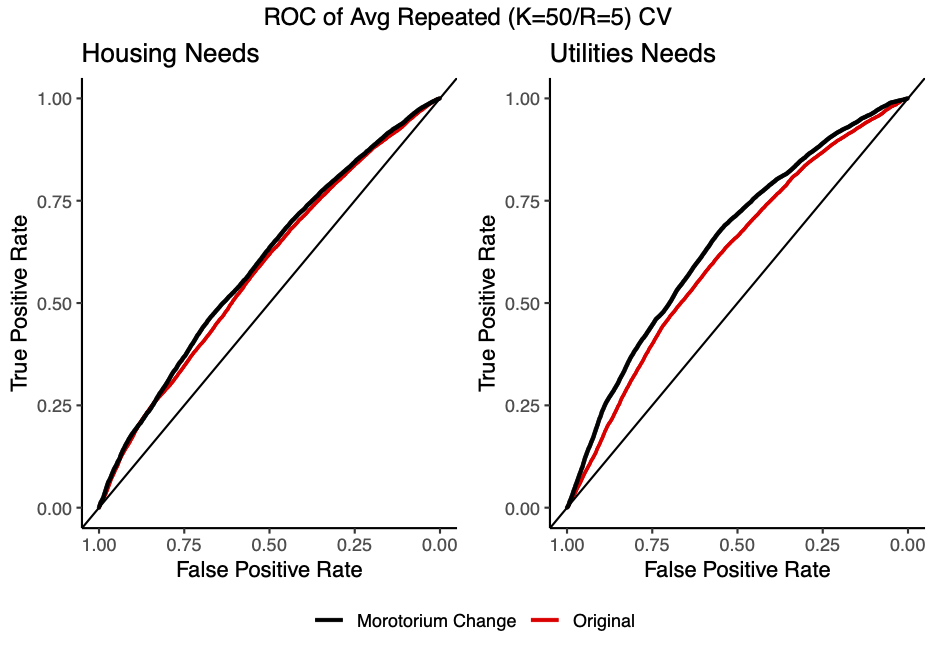
\includegraphics[width=0.7\linewidth]{figures/auc_roc_out_of_sample.png}
  %\caption{ROC/AUC Curve of Out-Of-Sample Model Performance for Logit Models | R = 5, K = 50.}
  \label{auc_roc_out_of_sample}
\end{figure}

\begin{table}[!htbp]
\centering
%\caption{AUC Scores}
\label{}
\scalebox{0.7}{
\begin{tabular}{ccc}
\\[-1.8ex]\hline
\hline \\[-1.8ex]
& $H_0$ & Moratorium Change Added \\
\hline \\[-1.8ex]
Housing Needs & $0.5839$ & $0.5984$ \\
Utilities Needs & $0.6138$ & $0.6496$ \\
\hline \\[-1.8ex]
\end{tabular}
}
\end{table}


\end{frame}



% Section 5
% What you learned from your project, and how your capstone host benefited from the work


\begin{frame}
\frametitle{Conclusion}
\framesubtitle{Evictions}

% CIE data is terrible for statistical analysis but potential in utility needs prediction

\begin{itemize}
	\item From this project we established clear differences in forced eviction rates before, during, and after the Covid-19 Moratorium for San Diego County.
	\item Forced evictions seem to be reverting to their prior state before moratorium protections
\end{itemize}

\end{frame}

\begin{frame}
\frametitle{Conclusion}
\framesubtitle{CIE Needs}

\begin{itemize}
	\item Data is not easily modeled.
	\item “Slight increase” in test scores unsatisfactory.
	\item Increase in observations, change in model type, recommended.
\end{itemize}

\end{frame}

\begin{frame}
\frametitle{Conclusion}
Only the starting point of future research to further investigate the relationship between the COVID-19 pandemic and housing instability.

\end{frame}



% End Slides (Extras)
\begin{frame}
\frametitle{}
\centering
\Huge Thank You!
\footnotetext{\url{github.com/AndyLAndrew/Homelessness_Hub_MS_CSS_Capstone}}
\end{frame}


\end{document}